\chapter{Choosing a City as an Entrepreneurial Constraint}

In this School of Hard Knocks segment, James presents a countdown of five cities for starting a business in 2021. We should read the list as more than a travel recommendation. A city changes the founder's constraint set: costs, clients, capital, network, talent, policy, and local culture all enter the operating conditions of a young business. This chapter follows the lecture's order and treats the ranking as a practical decision model, not as a formally measured index.

\paragraph{Source note.}
The spoken source is a School of Hard Knocks entrepreneurship video, curated for this book by LazyingArt LLC through Video2Book. No validated visual frames were retained for this lecture, so the figures below are transcript-derived reconstructions rather than screenshots of board work.

\section{The Ranking Problem}

James begins by telling us that the list is built from an ``accumulation'' of factors. The factors he names are opportunities, startup cost, cost of living, growth and profit potential, networking, and client opportunities. That opening is important: the unit of analysis is not simply a city, but an entrepreneurial environment.

A cautious way to write the decision problem is to let \(c\) denote a candidate city and to define a qualitative score
\begin{equation}
S(c)
=
w_oO(c)
+w_sS_c(c)
+w_lL(c)
+w_gG(c)
+w_nN(c)
+w_mM(c)
+w_kK(c)
+w_pP(c).
\end{equation}
Here \(O\) is opportunity, \(S_c\) is startup-cost condition, \(L\) is cost-of-living condition, \(G\) is growth and profit potential, \(N\) is network access, \(M\) is market or client access, \(K\) is capital access, and \(P\) is policy or tax condition. This is not a formula James calculates in the video. It is a clean notation for the reasoning he speaks through.

The countdown order is
\begin{equation}
\text{Seattle}=5,\qquad
\text{Denver}=4,\qquad
\text{Los Angeles}=3,\qquad
\text{Miami}=2,\qquad
\text{Austin}=1.
\end{equation}
The order matters because the lecture develops by tradeoff. We start with strong but costly ecosystems, then move toward places where the speaker sees more factors aligning at once.

\begin{figure}
\centering
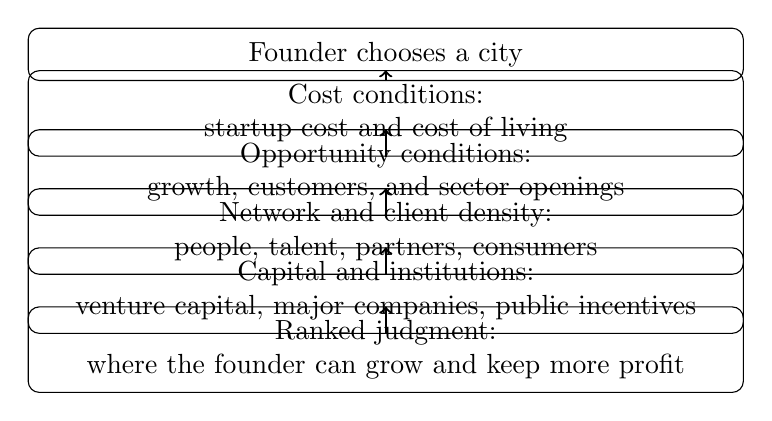
\begin{tikzpicture}[
  node distance=0.75cm,
  every node/.style={draw, rounded corners, align=center, text width=0.72\linewidth, inner sep=5pt},
  arrow/.style={->, thick}
]
\node (a) {Founder chooses a city};
\node (b) [below of=a] {Cost conditions:\\startup cost and cost of living};
\node (c) [below of=b] {Opportunity conditions:\\growth, customers, and sector openings};
\node (d) [below of=c] {Network and client density:\\people, talent, partners, consumers};
\node (e) [below of=d] {Capital and institutions:\\venture capital, major companies, public incentives};
\node (f) [below of=e] {Ranked judgment:\\where the founder can grow and keep more profit};
\draw[arrow] (a) -- (b);
\draw[arrow] (b) -- (c);
\draw[arrow] (c) -- (d);
\draw[arrow] (d) -- (e);
\draw[arrow] (e) -- (f);
\end{tikzpicture}
\caption{A transcript-derived decision flow. The lecture does not show this diagram, but its spoken ranking follows this cumulative logic.}
\end{figure}

\section{Seattle and Denver: Growth Meets Cost and Policy}

The countdown begins with Seattle. James describes it as one of the fastest-growing cities in the United States and as a city already known for technology. The newer point, in his framing, is that Seattle is becoming one of the country's fast-growing startup hubs. The counterweight is cost. Seattle has a high cost of living, but the speaker argues that a growing venture capital scene and economic development can offset some of the burden.

In the language of the score, Seattle is not winning by being cheap. It is winning enough to enter the list because its capital, tech base, growth, and entrepreneurial population are strong:
\begin{equation}
K(\text{Seattle})+G(\text{Seattle})+N(\text{Seattle})
\quad \hbox{partly offset} \quad
L(\text{Seattle}).
\end{equation}
The word ``partly'' is essential. The lecture does not claim cost disappears; it claims the ecosystem may compensate for it.

At number four, James moves to Denver. Denver is described as top ten both for starting a business and for startups. The argument changes slightly: where Seattle emphasizes technology and venture capital, Denver brings in government incentives and sector investment. The speaker names manufacturing, transportation, cannabis, and related industries as areas receiving multi-billion-dollar investment attention.

The Denver segment is somewhat garbled and repeated in the transcript, so the clean note is simple: Denver earns its place by combining livability, policy support, sector breadth, and appeal to young people who want to move, start, and progress.

\section{Los Angeles: Network Value Against High Cost}

Los Angeles appears at number three. James says it is one of the largest cities for tech entrepreneurship and the third largest city for startups in the United States. But this is also the place where the lecture's central tension becomes explicit: Southern California is expensive.

The speaker's answer is not to deny cost. He says, in effect, that network can change the calculation. Los Angeles has consumers, like-minded people, access to a broad market, and concentrated talent. Those things do not lower rent, but they can raise the ceiling on what a business can do.

\subsection{Question \& Answer}

\paragraph{Question.}
Why can an expensive city still rank highly for an entrepreneur?

\paragraph{Answer.}
Because cost is only one term in the founder's environment. A high-cost city may still be attractive if the network, market, talent, and client access are strong enough to improve the business's chances of growth. In compact form, the Los Angeles argument is
\begin{equation}
N(c)+M(c)+G(c)+K(c)
\quad \hbox{can outweigh} \quad
L(c)
\end{equation}
when the city gives a founder access to people, customers, capital, and demand that would be harder to reach elsewhere.

This is the lecture's most useful local obstacle. If we flattened the ranking into a cheap-versus-expensive comparison, Los Angeles would be hard to explain. But the spoken reasoning is ecosystem reasoning: a market full of consumers and builders may justify staying in a costly place, though not enough, in James's ranking, to move Los Angeles above number three.

\section{Miami: Density, Collaboration, and Institutional Support}

The move from Los Angeles to Miami is a move from network value to density. James calls Miami an incredible place to start a business and says it has the highest density of startups in the country. He also emphasizes creativity, opportunity, and collaboration: a city full of people and a city where businesses can innovate, develop, and grow.

The concrete institutional claim is that Miami has 139 Inc. 5000 companies located there:
\begin{equation}
\#\{\hbox{Inc. 5000 companies in Miami}\}=139.
\end{equation}
He also points to venture capital support and says Miami ranks as a top-five fastest-growing city in the United States. The logic is cumulative. Miami is not described through one decisive variable; it is described as a cluster of reinforcing supports:
\begin{equation}
S(\text{Miami})
\approx
\hbox{startup density}
+\hbox{collaboration}
+\hbox{institutional support}
+\hbox{capital}
+\hbox{city growth}.
\end{equation}
Again, the equality is not a calculation. It is a disciplined shorthand for the mechanism the transcript gives us.

\section{Austin: The Combined Case for Number One}

The final pivot is to Austin, Texas. James presents Austin as the number-one city on his list. The evidence comes in a sequence: fastest-growing city in the United States, ranked by CNBC as the number-one city to start a business in 2021, startup growth of 81 percent, innovation, technology, startup culture, affordability, consumer availability, networking, no state income tax, zero percent corporate tax rate as stated, and a supportive culture for entrepreneurs and small businesses.

The spoken quantitative claims are
\begin{equation}
\hbox{Austin startup growth}=81\%,
\end{equation}
and, as James states them,
\begin{equation}
\hbox{state income tax}=0,
\qquad
\hbox{corporate tax rate}=0\%.
\end{equation}
These tax statements should be kept as speaker-attributed claims, not as tax advice. Their role in the lecture is clear: policy and retained profit are part of the attractiveness of place.

\paragraph{Worked example: a qualitative score update.}
Suppose we begin with a neutral city score \(S_0(c)\). As James adds evidence, we can think of the score being updated by factors rather than computed from hard data:
\begin{align}
S_1(c) &= S_0(c)+\Delta_{\text{growth}}(c),\\
S_2(c) &= S_1(c)+\Delta_{\text{network}}(c)+\Delta_{\text{clients}}(c),\\
S_3(c) &= S_2(c)+\Delta_{\text{capital}}(c)+\Delta_{\text{institutions}}(c),\\
S_4(c) &= S_3(c)+\Delta_{\text{policy}}(c)-\Delta_{\text{cost}}(c).
\end{align}
For Austin, the speaker's conclusion is that the positive increments dominate: growth, startup culture, affordability, taxes, consumer availability, network opportunity, and supportive local culture all point in the same direction.

\section{The Ranking as a Compact Table}

The lecture is not a spreadsheet, but the spoken evidence is compact enough to organize in a table. The entries below preserve the countdown order and keep the claims tied to the speaker's framing.

\begin{table}
\centering
\begin{tabular}{c|p{0.18\linewidth}|p{0.33\linewidth}|p{0.31\linewidth}}
Rank & City & Main stated advantages & Constraints or concrete claims \\
\hline
5 & Seattle &
Tech hub; fast-growing startup hub; growing venture capital scene; young and innovative crowd &
High cost of living, partly offset in the speaker's view by economic development and capital access \\
\hline
4 & Denver &
Top-ten business and startup city; tax incentives; investment across manufacturing, transportation, cannabis, and more &
Transcript segment repeats and is partly garbled; consolidate as policy plus sector opportunity \\
\hline
3 & Los Angeles &
Large tech entrepreneurship city; third largest startup city; consumers, talent, global market access, and network density &
Very high cost of living keeps it at number three \\
\hline
2 & Miami &
Highest startup density claim; creative and collaborative city; institutional support; venture capital support &
Speaker states 139 Inc. 5000 companies and top-five fastest-growing-city status \\
\hline
1 & Austin &
Fastest-growing city claim; CNBC number-one claim; startup culture; affordability; networking; supportive business culture &
Speaker states 81 percent startup growth, no state income tax, and zero percent corporate tax rate \\
\end{tabular}
\caption{Transcript-backed ranking evidence, arranged for compact note use.}
\end{table}

\section{Summary}

The lecture's practical lesson is that location is part of entrepreneurship strategy. We are not merely asking where it is pleasant to live or where rent is lowest. We are asking where opportunity, cost, network, customers, capital, institutions, taxes, and culture combine in a way that lets a business start and grow.

The countdown preserves that logic. Seattle introduces tech gravity and venture capital against cost. Denver adds policy and sector investment. Los Angeles makes the central tradeoff unavoidable: high cost can be rational if network and market access are strong. Miami adds density, collaboration, institutions, and capital. Austin closes the ranking by combining growth, affordability, policy advantages, and supportive startup culture into the speaker's number-one choice.